\chapter{}
Jetzt etwas für Bastelenthusiasten.
Wenn wir eine Metrik haben, dann können wir eine Topologie basteln. 
Hirfür definieren wir die Menge:
$$Z : U_{x,l }:= x + l\mathbb{Z} = \{x + ln \mid n \in \mathbb{Z}\}, x \in \mathbb{Z}, l\in \mathbb{Z}, l \ge 1$$.

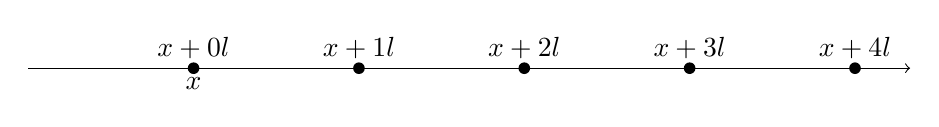
\begin{tikzpicture}[scale=0.7]
  % Parameter
  \def\x{2}   % Startwert
  \def\l{3}   % Schrittweite

  % Zahlengerade
  \draw[->] (-1,0) -- (15,0);

  % Punkte U_{x,l} = {x + l n}
  \foreach \n in {0,...,4}{
    \pgfmathsetmacro{\wert}{\x+\l*\n}
    \fill (\wert,0) circle (3pt)
      node[above] {$x+{\n}l$};
  }

  % Den Startwert extra beschriften
  \node[below] at (\x,0) {$x$};

\end{tikzpicture}

Das ganze ist sehr lustig, also unanschaulich. Also lustig für Mathematiker halt. 
Es kann natürlich sein das einem der Witz an dem ganzen bis dato noch nicht aufgefallen ist. 
Aber nach dem man darauf aufmerksam gemacht wurde, ist es sehr lustig.
\bigskip

Betrachten wir also die Topologie:
$$\mathcal{T} := \{ O \subseteq \mathbb{Z} \mid \forall x \in O \exists l \in \mathbb{Z}, l \ge 1 : U_{x,l} \subseteq O\}$$
\begin{itemize}
    \item Sei $U_{k,l} \in \mathcal{T}, x \in U_{k,l}$. \\
    Dann gilt: $U_{x,l}=U_{k,l} : \text{ endlich}$
    Denn mit $n_x \in \mathbb{Z}: x = k + n_x l$. erhalten wir: \\
    \begin{itemize}
        \item Sei $y \in U_{x,l}: y = x + n_y l = U_{k,l} \ni k + (n_x + n_y)l$.
        \item Sei $y \in U_{k,l}: y = k + n_y l = U_{x,l} \ni x + (n'_y - n_{x})l$.
    \end{itemize}

    \item Das folgende ist eine Mengenspielerei und zur Erinnerung: Das gefällt uns!\\
    Wir betrachten also die Menge $$\mathbb{Z} \setminus U_{k,l} \in \mathcal{T}: \mathbb{Z} \setminus U_{k,l} 
    = \underset{x= k+1}{\overset{k+l-1}{\bigcup}} U_{x,l} \in \mathcal{T}$$
    Und weiters 
    $$\mathbb{Z}\setminus\{1,-1\} = \underset{p \in \mathbb{P}}{\bigcup} U_{0,p} \dots \{1,-1\}$$
    Hir ist wichtig zu bemerken, dass die Geometrische Progession unendlich ist und die Menge $\{-1,1\}$ nicht. 
    Das bedeutet $\{1,-1\} \notin \mathcal{T}$.\\
    $= \underset{p \in \mathbb{P}}{\bigcup}\underset{\in \mathcal{T}}{\mathbb{Z}\setminus{U_{0,p}}}$. 
    $\mathbb{P}:= \{p \in \mathbb{N} \mid p \text{ Prim} \,\} \Rightarrow \mathbb{P} \text{ unendlich}$.
    Damit haben wir auch gezeigt, dass die Menge der Primzahlen unendlich ist.
    
\end{itemize}

\dfn{Halbordnung auf der Menge der Topologien}{

Sei $X$ eine Menge. 
Betrachte 
$$
\mathbb{T}(x) := \{\mathcal{T}(X)\subset \mathcal{P}(X)\mid \mathcal{T} \text{ Topologie auf } X\}
$$  
Die Potenzmenge einer Menge ist in natürlicher Weise halbgeordnet 
durch die Teilmengenbeziehung $\subseteq$. 
Damit ist auch $\mathbb{T}(X)$ halbgeordnet durch $\subseteq$. Konkreter definieren wir 
 $\mathbb{T}(X)$ ist eine halbgeordnet mit $\subseteq$ 
  Seien $\mathcal{T}_1, \mathcal{T}_2 \in \mathbb{T}(x)$
  Dann ist $\mathcal{T}_1 \subseteq \mathcal{T}_2$ eine Hablbordnung mit: 
  $$
  \forall O \subseteq X: O \in \mathcal{T}_1 \Rightarrow \mathcal{T}_2
  $$
\nt{
\dfn{Feinheit}
{
Sei $X$ eine Menge, und $\mathcal{T}, \mathcal{V} \in \mathbb{T}(X)$.  
\textit{Wir sagen $\mathcal{T}$ ist \emph{feiner} als $\mathcal{V}$, wenn $\mathcal{V} \subseteq \mathcal{T}$, 
und sagen $\mathcal{T}$ ist \emph{gröber} als $\mathcal{V}$, wenn $\mathcal{T} \subseteq \mathcal{V}$.}
}
}
}

Weiters schauen wir uns noch zwei Eigenschaften von $\mathbb{T}(X)$ an .

\begin{itemize}
  \item $\{\emptyset, X\} \in \mathbb{T} \text{ und } \forall \mathcal{T} \in \mathbb{T}:
  \{\emptyset,X\}\subset \mathcal{T}$ so wie 
  $\mathcal{P}(X) \in \mathbb{T}(X) $ und $\forall \mathcal{T} \in \mathbb{T}(X): \mathcal{T}\subset \mathbb{P}$
  \item $\mathbb{V} \subseteq \mathbb{T}(X)$ Dann gilt: $\mathbb{V} \neq \emptyset\footnote{\text{ um Sonderfälle zu vermeiden}}$ 
  hat ein Infimum in $\mathbb{T}(X)$.
\end{itemize}
Die erste Eigenschaft geht aus vorherigen Beobachtungen hervor. 
Die zweite Eigenschaft bedarf etwas mehr Arbeit.

\begin{proof}
  Wir wollen zeigen, dass jede nichtleere Teilmenge von $\mathbb{T}(X)$ ein Infimum hat.
 \begin{enumerate}
    \item Im ersten Schritt wählen wir einen Kandidaten  $\mathbb{V}$ in $\mathbb{T}(X)$ 
    Hierfür betrachten wir $\bigcap \mathbb{V} \in \mathbb{T}(X)$
    \begin{itemize}
      \item Sei $V \in \mathbb{V}$ dann ist 
      $\emptyset \in V$ und $X \in V \Rightarrow \emptyset \in \bigcap \mathbb{V}$
      und damit auch $x \in \bigcap \mathbb{V}$ 
      \item Betrachte weiters $\mathcal{V} \subseteq \bigcap \mathbb{V}$ und $V \in \mathbb{V}$. 
      Dann gilt:
      $$ 
      \mathcal{V} \subseteq V \Rightarrow \bigcup \mathcal{V} \in V \Rightarrow \bigcup \mathcal{V} \in \bigcap \mathbb{V}.
      $$
      \item
      $\mathcal{V} \subseteq \bigcap \mathbb{V}$ endlich und sei $V \in \mathbb{V}$. 
      Dann gilt:
      $$ 
      \mathcal{V} \subseteq V \Rightarrow \bigcap \mathcal{V} \in V \Rightarrow \bigcap \mathcal{V} \in \bigcap \mathbb{V}.
      $$
    \end{itemize}
    Damit sehen wir, dass unser gewählter Kandidat in der Grundmenge ist - was ihn zu einem guten Kanditaten macht -.
    (Hier Politik Bashing einfügen - da, da gibt es zu meist keinen guten Kandidaten etc. -) 

    \item Im nächsten Schritt zeigen wir, dass $\bigcap \mathbb{V}$ eine Untere Schranke ist:\\
   Sei $\mathcal{V}  \in \mathbb{V} $ dann gilt $\bigcap \mathbb{V} \in \mathbb{T}(X)$ \\
   Mit  $\mathcal{V}  \in \mathbb{V} :$ fehlt zu zeigen, dass $\mathcal{V} \subseteq \bigcap \mathbb{V}$.
   Was direkt daraus folgt das $V \in \bigcap \mathbb{V} :$ da $V \in \mathcal{V}$

    \item Wir zeigen jetzt noch, dass $\bigcap \mathbb{V}$ nicht nur irgend eine untere Schranke ist,
    sondern die Größte.\\
    Sei $\mathcal{W} \in \mathbb{T}(X)$ eine untere Schranke von $\mathbb{V}$
     - hier irgend eine untere Schranke - und fragen uns:
    Was bedeutet es, eine untere Schranke zu sein?
    $$\forall V \in \mathbb{V}: \mathcal{W} \subseteq V$$
    Zu zeigen ist noch: $\mathcal{W} \subseteq \bigcap \mathbb{V}$.
    Das heißt $\forall \mathcal{V} \in \mathbb{V}: \mathcal{W} \subseteq \mathcal{V}$.
    Das heißt wiederum $\forall \mathcal{V} \in \mathbb{V}, \forall O \in \mathcal{W}: O \in \mathcal{V}$.
    also $\forall O \in \mathcal{W}: O \in \bigcap \mathbb{V}$.
    Das heißt $\mathcal{W} \subseteq \bigcap \mathbb{V}$.
  \end{enumerate}
\end{proof}


\nt{ Jede Menge, die ein Infimum hat und ein größtes Element, dann hat jede Teilmenge auch ein Supremum.}

An der Bemerkung angelehnt, wollen wir jetzt noch zeigen, dass jede Teilmenge von $\mathbb{T}(X)$ auch ein Supremum hat.

\nt{
\begin{corollary}{Jede Teilmenge von $\mathbb{T}(X)$ hat ein Supremum. }
  Vergleichen wir das mit der Eigenschaft das $\mathbb{V} \subseteq \mathbb{T}(X)$ ein Infimum hat.
  Dan Wäre dsa Äquivallent das die vereinigung der Topologien das Supremum ist. 
  Aber im Algemeinen ist die Vereinigung von Topologien keine Topologie.
\end{corollary}
}

\mprop{}{
  Sei $X$ eine Menge und sei $\mathcal{S}
  \footnote{ Weil S oder $\mathcal{S}$ macht keinen Unterschied - Die Begründung begründet etwas -} 
  \subseteq \mathcal{P}(X)$. Dann ist 
  $$ \mathcal{\bigstar} :=
  \left\{
    \bigcup_{i \in I} \bigcap_{j = 1}^{n_i} O_{ij} 
    \,\middle|\,
    I \text{ Menge},\; n_i \in \mathbb{N},\; O_{ij} \in \mathcal{S}
  \right\}.
$$
eine Topologie
}
\begin{proof}{Proposition: 2.0.4:}\\

  \begin{itemize}
    \item[(O1)] $\emptyset, X \in \mathcal{T}$.
    Folgt direkt aus $\mathbb{I} = \emptyset \Rightarrow \emptyset$ 
    und $n_i = 0 \Rightarrow X$ ,
    \item[(O2)] Sei $V \subseteq \mathcal{T}$ endlich, dann gilt $V = \emptyset: \bigcap V = X$
    \item[(O3)] Es fehlt zu zeigen, dass $\mathcal{T}$ 
    unter endlichen Durchschnitten abgeschlossen ist. Seien also
    \begin{equation*}
      \bigcup_{i \in I_k} \bigcap_{j = 1}^{n_{ik}} O_{ijk} \in \mathcal{T}, 
      \quad k = 1, \dots, m.
    \end{equation*}
    Dann gilt
    \begin{equation*}
      \bigcap_{k = 1}^{m} 
      \left[
        \bigcup_{i \in I_k} \bigcap_{j = 1}^{n_{ik}} O_{ijk}
      \right]
      =
      \bigcup_{(i_1, \dots, i_m) \in I_1 \times \dots \times I_m}
      \left(
        \bigcap_{j = 1}^{n_{i_1 1}} O_{i_1 j 1}
        \cap \dots \cap
        \bigcap_{j = 1}^{n_{i_m k}} O_{i_m j k}
      \right)
    \end{equation*}
    und diese Menge ist wieder eine Vereinigung von endlichen Durchschnitten von Mengen aus 
    $\mathcal{S}$,  
    gehört also zu $\mathcal{T}$.
  \end{itemize}
\end{proof}


\mlenma{$\bigstar$ Ist die kleinste Topologie, die $\mathcal{S}$ enthält.}
{
Sei $X$ eine Menge und sei $\mathcal{S} \subseteq \mathcal{P}(X)$. 
Dann ist $\bigstar$ die kleinste \footnote{Die gröbste} Topologie, die $\mathcal{S}$ enthält
}
\begin{proof}{Lemma 2.0.5: }\\
  jede Topologie, die $\mathcal{S}$ umfasst, muss auch $\mathcal{T}$ umfassen.  
  Also ist $\bigstar \subseteq \mathcal{T}$.
\end{proof}


\begin{corollary}{}
  aSei $\mathbb{V} \subseteq \mathbb{T}(X)$.  
  Dann ist $\sup \mathbb{V}$ die von $\bigcup \mathbb{V}$ erzeugte Topologie.
\end{corollary}

\begin{proof}{Korollar 2.0.6:}\\
  \begin{equation*}
  \forall \mathcal{V} \in \mathbb{V} : 
  \sup \mathbb{V} \ge \mathcal{V}\Rightarrow
  \sup \mathbb{V} \supseteq \bigcup \mathbb{V}\Rightarrow
  \sup \mathbb{V}  \ge \mathcal{R}.
  \end{equation*}
\end{proof}

\dfn{Stetig}
{
Seien $(X, \mathcal{T}), (Y, \mathcal{V})$ topologische Räume, und $f : X \to Y$ eine Funktion.  
Dann heißt $f$ \textbf{stetig}, wenn
\begin{equation*}
  \forall O \in \mathcal{V} : f^{-1}(O) \in \mathcal{T}.
\end{equation*}

Muss man sich spezifischer ausdrücken, so sagt man auch:  
$f$ ist $\mathcal{T}$–$\mathcal{V}$–stetig.\footnote{ An diesem Punkt ist es 
angebracht, Panik zu bekommen, da wir hier den Begriff der Stetigkeit mit einer zweiten
Definition belegen}

}
\subsection{Einschub: Metrik}

Welche Begriffe kennen wir? - das wir $\setminus\{\text{Woracheck}\}$-
(Er kennt vermutlich auch noch viele andere Begriffe, von denen wir bis jetzt noch 
"verschont geblieben" sind.)

\begin{itemize}
  \item konvergente Folge

  \item $A \subseteq X$.  
  Der \textbf{Innere} von $A$ (=: $\r{A} $) ist
  \begin{equation*}
    \operatorname{int}(A) = \{ x \in A \mid \exists r > 0 : U_r(x) \subseteq A \}.
  \end{equation*}

  \item $A \subseteq X$ heißt \textbf{offen} $\Leftrightarrow A = \r{A}$.

  \item $A \subseteq X$ heißt \textbf{abgeschlossen} $\Leftrightarrow A = \overline{A}$.

  \item $A \subseteq X$ heißt \textbf{Abschluss} von $A$ ($\overline{A}$) ist
  \begin{equation*}
    \overline{A} = \{ x \in X \mid \forall r > 0 : U_r(x) \cap A \neq \emptyset \}.
  \end{equation*}

  \item $\partial A = \overline{A} \setminus \r{A}$.

  \item $(X, d_X), (Y, d_Y)$ metrische Räume, $f : X \to Y$ heißt \textbf{stetig} $\Leftrightarrow$
  \begin{equation*}
    \forall \varepsilon > 0 \; \exists \delta > 0 : 
    \forall x, x' \in X :
    d_X(x, x') < \delta \;\Rightarrow\; d_Y(f(x), f(x')) < \varepsilon.
  \end{equation*}

  \item $A \subseteq X$ heißt \textbf{kompakt} $\Leftrightarrow$ 
  jede offene Überdeckung $(O_i)_{i \in I}$ von $A$ besitzt eine endliche Teilüberdeckung, d.\,h.
  \begin{equation*}
    A \subseteq \bigcup_{i \in I} O_i 
    \;\Rightarrow\;
    \exists I_0 \subseteq I \text{ endlich mit } A \subseteq \bigcup_{i \in I_0} O_i.
  \end{equation*}

  \item \textbf{Satz:}  
  $f$ ist stetig $\Leftrightarrow \forall A \subseteq Y$ offen $\Rightarrow f^{-1}(A)$ offen.
\end{itemize}

\subsection{Definitionen in topologischen Räumen}

\dfn{Offen und abgeschlossen}
{
  Sei $\langle X, \mathcal{T} \rangle$ ein topologischer Raum.  
  \begin{itemize}
  \item $A \subseteq X$ heißt \textbf{offen} $:\Leftrightarrow A \in \mathcal{T}$.
  \item $A \subseteq X$ heißt \textbf{abgeschlossen} $:\Leftrightarrow X \setminus A$ offen.
  \end{itemize}
}

\mlenma{Lemmachen}{
 
Sei $\langle X, \mathcal{T} \rangle$ topologisch und $A \subseteq X$.

\begin{enumerate}
  \item $\bigcup \{ O \subseteq X \mid O \in \mathcal{T},\, O \subseteq A \}$  
  ist die größte offene Menge, die in $A$ enthalten ist.
  \item $\underbrace{\bigcap \{ C \subseteq X \mid X \setminus C \in \mathcal{T},\, A \subseteq C \}}_{\text{Dieser}}$
  ist die kleinste abgeschlossene Menge, die $A$ umfasst.
\end{enumerate}
}

%%%%%%%%%%%%%%%%%%%%%%Sketchy$$$$$$$$$$$$$$$$

\begin{proof}{Lemma 2.1.3: }\\
\begin{enumerate}
  \item[(ii)+(iii)]  
  $\forall C$ aus \textbf{Dieser} Menge halt:  
  Erfüllt $C \supseteq A$, so gilt auch $\bigcap \{C\dots\} \supseteq A$.  

  Denn:  
  $X \setminus \bigcap \{C) \subseteq X \setminus A$.  
  Also ist $\bigcap C \supseteq A$.

  Sei $D \subseteq X$, sodass $D \supseteq A$.  
  $\Rightarrow D$ kann noch in $\bigcap C$ enthalten sein.
\begin{equation*}
X \setminus \bigcap_{C \in \mathcal{C}} C 
= \bigcup_{C \in \mathcal{C}} (X \setminus C)
\subseteq X \setminus A
\Rightarrow
\bigcap_{C \in \mathcal{C}} C \supseteq A.
\end{equation*}

Sei $D \subseteq X$, also $D \supseteq A$.  
$$
\Rightarrow D \text{ kann nur in } \bigcap_{C \in \mathcal{C}} C \text{ enthalten sein.}
$$
\end{enumerate}
\end{proof}
%%%%%%%%%%%%%%%%%%%%%%%%%%%%%%%%%%%%%%%%%%%%%%%%%%%%%%%%%

\dfn{Innere, Äußere und Rand}
{
\begin{itemize}
\item Das \textit{Innere} $B^{\circ}$ einer Teilmenge $B$ eines topologischen Raumes $(X, \mathcal{T})$
ist definiert durch
$$
   \mathring{B} = \bigcup \{\, O \in \mathcal{T} : O \subseteq B \,\}.
$$
\item Das \textit{Äußere} $B^{\circ}$ einer Teilmenge $B$ eines topologischen Raumes $(X, \mathcal{T})$
ist definiert durch
$$
   \bar{B} = \bigcap \{\, C \subseteq X : X \setminus C \in \mathcal{T},\, B \subseteq C \,\}.
$$
\item Der \textit{Rand} $\partial B$ einer Teilmenge $B$ eines topologischen Raumes $(X, \mathcal{T})$
ist definiert durch
$$
  \partial B = \bar{B} \setminus  \mathring{B}.
$$
\end{itemize} 
}

\dfn{kompakt}
{
  Eine Teilmenge $K$ eines topologischen Raumes $(X, \mathcal{T})$ heißt \textbf{kompakt},  
wenn jede offene Überdeckung von $K$, also $\mathcal{V} \subseteq \mathcal{T}$ mit
\begin{equation*}
  \bigcup_{V \in \mathcal{V}} V \supseteq K,
\end{equation*}
eine endliche Teilüberdeckung besitzt, es also $V_1, \ldots, V_n \in \mathcal{V}$ gibt mit
\begin{equation*}
  V_1 \cup \dots \cup V_n \supseteq K.
\end{equation*}

Eine Teilmenge $A \subseteq X$ heißt \textbf{relativ kompakt},  
wenn $\operatorname{cl}(A) \subseteq X$ kompakt ist.

Sei $\mathcal{C}$ eine Familie von Teilmengen einer Menge $X$, also $\mathcal{C} \subseteq \mathcal{P}(X)$.  
Wir sagen, dass $\mathcal{C}$ die \textbf{endliche Durchschnittseigenschaft} hat,  
wenn für je endlich viele $C_1, \ldots, C_n \in \mathcal{C}$ stets
\begin{equation*}
  C_1 \cap \dots \cap C_n \neq \emptyset
\end{equation*}
gilt.
}

\thm{Zusammenhang Zwischen Metrischen und Topologischen Räumen}
{
Sei $\langle X,d \rangle $ ein metrischer Raum. Dann betrachte den Topologischen Raum $\langle X, \mathcal{T}_d \rangle$ mit.
Dann sind alle Begriffe die wir in metrischen Räumen definiert haben auch in topologischen Räumen definiert.
\begin{itemize}
  \item $\forall A \subseteq X:$ A ist offen im Metrischen Sinne $\Leftrightarrow A $ ist offen im topologischen Sinne
  \item usw
\end{itemize}
}
